\documentclass[final,6p,times,twocolumn,authoryear]{elsarticle}
\usepackage{amssymb}
\usepackage{amsmath}
\usepackage{lipsum}
\usepackage{graphicx}
\usepackage{tabularx}
\usepackage{wrapfig}
\journal{School of Information, UC Berkeley}


\begin{document}

\begin{frontmatter}

\title{Generalized Soft Prompt Transfer}

\author[berkeley]{Aswin Thiruvengadam}
\author[berkeley]{Hannah George}
\author[berkeley]{Raul Merino}
\affiliation[berkeley]{organization={University of California, Berkeley}}

\begin{abstract}
\begin{wrapfigure}{r}{0.45\textwidth}
    \centering
    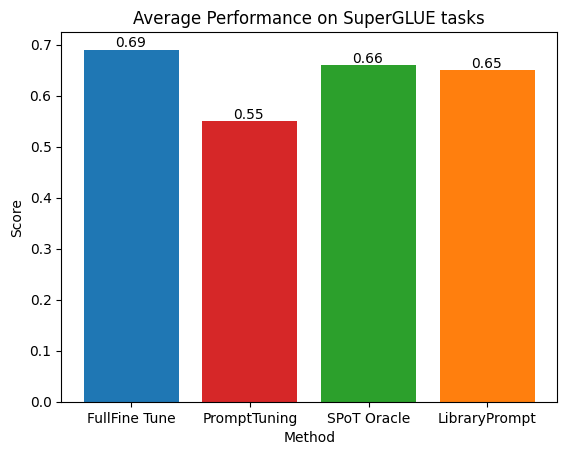
\includegraphics[width=0.45\textwidth]{bar_chart_results.png}
\end{wrapfigure}
This paper introduces a new method for transfer learning in natural language processing (NLP) which we have called LibraryPrompt. The proposed approach builds on the success of soft prompt transfer methods (SPoT), which have shown remarkable performance on a variety of NLP tasks. However, SPoT requires knowledge of the degree of task similarity between the source and target tasks, which can be time-consuming and may not generalize well to new tasks. In contrast, LibraryPrompt does not need to have any information about the similarity between target and source tasks, as it’s constructed from a library of learned prompts from a variety of different NLP tasks.

Using the GLUE dataset for the source tasks, we constructed the library of learned prompts for LibraryPrompt. We evaluated it on several SuperGLUE tasks and found that it performed well with a score of 65\%, outperforming vanilla prompt-tuning (55\%) and scoring similarly to SPoT (66\%) using the same GLUE tasks as the source tasks, despite not having any prior information about the target tasks.

Overall, our results suggest that LibraryPrompt is a promising direction for transfer learning in NLP, and has the potential to reduce the time needed for successful prompt tuning.
\end{abstract}

%%Graphical abstract
%\begin{graphicalabstract}
%\includegraphics{grabs}
%\end{graphicalabstract}

%%Research highlights
%\begin{highlights}
%\item Research highlight 1
%\item Research highlight 2
%\end{highlights}

% \begin{keyword}
%% keywords here, in the form: keyword \sep keyword
% keyword \sep keyword \sep keyword \sep keyword

%% PACS codes here, in the form: \PACS code \sep code

%% MSC codes here, in the form: \MSC code \sep code
%% or \MSC[2008] code \sep code (2000 is the default)

% \end{keyword}


\end{frontmatter}
% \tableofcontents

%% \linenumbers

%% main text

\section{Introduction}
Training large models - particularly large language models - can involve billions of trainable parameters. Fine-tuning these pre-trained models for specific downstream tasks requires significant computational resources. Due to this limitation of fine-tuning such models, researchers have been exploring solutions that reduce the number of parameters during the fine-tuning stage. Several methods have been proposed such as adapters \citep{houlsby_2019}, prompt tuning \citep{lester_2021}, p-tuning \citep{liu_2021},  prefix tuning \citep{li_2021} and LoRA \citep{hu_2021}. Studies on prompt-based methods in particular have shown that learned prompts can be effectively transferred between similar tasks \citep{vu_2022} by initializing the prompts for a new task with the learned prompts from a previous similar task. However, these transfer methods require knowledge of the degree of task similarity between the source and target tasks to determine the appropriate weights for the transfer \citep{vu_2022}. In this work we demonstrate a generic solution that allows for weights to be transferred during fine tuning without the need for a task similarity metric.

\begin{figure*}[t]
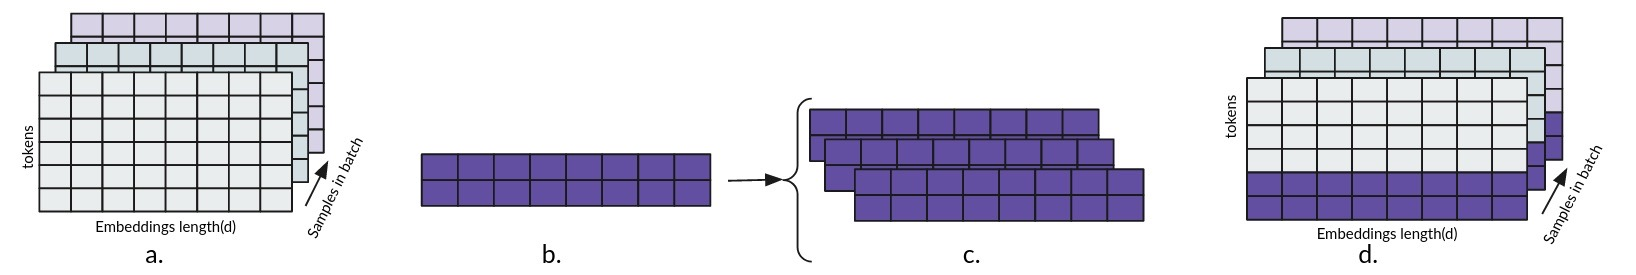
\includegraphics[width=\textwidth]{embeddings.jpeg}
\caption{a) The input embeddings have the shape of batch size $\times$ tokens $\times$ embeddings length ($d=768$). b) A trainable layer of weights of size $n=20$ $\times$ embedding length ($d=768$) is created. c) The trainable layer is replicated to match the batch size. d) The first $n$ tokens from the input are eliminated and replaced with these embeddings.}
\label{embeddings}
\centering
\end{figure*}


\section{Methodology}
The pre-trained model for our evaluation is an LM adapted T5 model \citep{lester_2021}, accessed through HuggingFace. We evaluated the model on the GLUE (General Language Understanding Evaluation) and SuperGLUE (Super General Language Understanding Evaluation) classification tasks. The two parameters that we pre-determined were the decoder max length and the beam length. We set the decoder max length to the number of max answer tokens plus one, and we set the beam length to the number of class labels.

The data preparation for the encoder of the fully fine-tuned models follows the text-to-text methodology used by \cite{raffel_2022}. The only exception is the SuperGlue WSC dataset, which did not follow the paper. This was a change that was observed late in development and hence kept. Preparation for a sample dataset for each of the tasks is shown in the appendix. Our implementation of the soft prompt simply eliminates the input embeddings for the first $n$ tokens and replaces them with trainable parameters (Figure \ref{embeddings}). For this reason the encoder input text for the soft prompt models are concatenated with $n$ words. We chose the word "absence" for this but any word with a one token representation could have been used instead. As a design choice these evaluations have all been conducted for a token length of $n=20$ tokens.

In order to construct the generic solution we needed to obtain the learned prompts for a variety of NLP tasks. We used the GLUE as the source tasks and SuperGLUE benchmark datasets. SuperGLUE tasks tend to have fewer samples than the GLUE tasks and hence were chosen as the target for prompt transfer.  These tasks cover a range of NLP objectives, including sentiment analysis, natural language inference, and question answering. We chose only a subset of tasks related to classification for this evaluation. The benchmark data are available as train and validation datasets. We further split the validation into a 60-40 dataset with 40\% allocated as an unseen test set. All performance numbers quoted in this paper are for this test set. The seeds for the shuffling of the dataset before splitting is changed for every repeat run of the experiment to get a better estimate of the mean performance across tests.


\section{Baseline}
We first started by establishing our baselines with fully fine tuned models where all the parameters of the model are trained for each GLUE and SuperGLUE benchmarks.  We then compare the performance of vanilla soft prompt tuning (PromptTuning) \citep{lester_2021} on these benchmarks. We first initialize the prompts with the tokens associated with the labels of the answer and any tokens that are not filled with the answer labels are initialized to a random word chosen from the 300 most common words in the train set for the task. For the prompt transfer experiments, we ran every target SuperGLUE task for every GLUE source task. The performance numbers hence quoted are the best across all source tasks. We used the same terminology as \cite{vu_2022} and called it the oracle (SpoT Oracle).

\begin{figure*}[t]
\centering
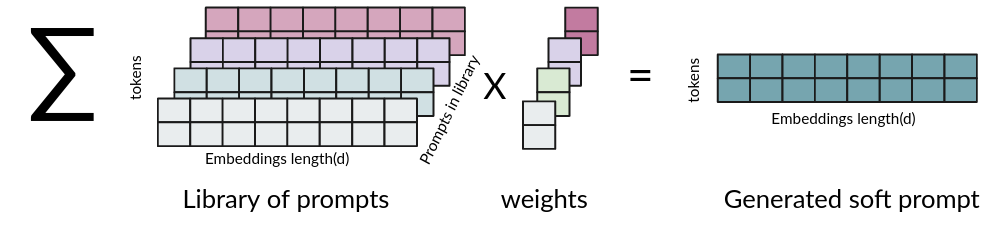
\includegraphics[width=0.6\textwidth]{library_prompts_cross_weights.png}
\caption{Generalized soft token is a weighted average of the library prompt. The size of the weight matrix is prompts $\times$ tokens. 
$$\overrightarrow{e}_t=\sum_p w_{p,t} \cdot \overrightarrow{e}_{p,t}$$ Where $t$ is one of $n$ tokens, $p$ is one of $P$ prompts in the library, $w_{p,t}$ is a trainable weight for each token of a library prompt, $\overrightarrow{e}_t$ is an embedding vector in the soft prompt, and $\overrightarrow{e}_{p,t}$ is the embedding vector for the token $t$ and prompt $p$ in the library.}
\label{library_prompts_cross_weights}
\end{figure*}


\section{Generalized Soft Prompts}
In the case of soft prompt transfer \citep{vu_2022}, one pre-trained soft prompt is loaded during initialization and fine tuned on the target task. Its performance on the target task was shown to be correlated to the cosine similarity of the target task embeddings and the source task embeddings. As the target tasks embeddings are only known after the model has been fine tuned for a certain number of steps on the target task, a retrieval system was designed which performs the cosine similarity and retrieves the appropriate source task. In our implementation, we created a library of source tasks and compared different methods of generating the embedding directly from this library when training on the target task. The best performing architecture - amongst those evaluated - is shown in Figure \ref{library_prompts_cross_weights} where a set of weights associated with each prompt and token along with the library are trained. As an example, for a library of 8 pre-trained prompts with 20 tokens and an embedding size of 768, this would be a total of $8 \times 20 + 8 \times 20 \times 768=123,040$ trainable parameters. As the library is trainable, this substantially increases the number of trainable parameters.  It is important to note that these trainable parameters are hidden behind the 20 soft tokens and do not participate in the attention calculations of the T5 model.


\section{Training}
All models were trained with a batch size of 32 for 30,000 steps. The Adam Optimizer, specifically the AdamW implementation on Tensorflow was used with the parameters $\beta_1=0.8$, $\beta_2=0.999$, and weight decay = 1E-5. The learning rate for PromptTuning and LibraryPrompt was set to 0.3 and for SPoT it was set to 0.1.  The learning rates for FullFineTuning were customized per dataset as a single learning rate did not work well for all datasets. For determining this learning rate, a single epoch of training was run where each batch received an increasing learning rate from 1E-7 to 1. For each step of this batch, the loss was measured. At the end of training, the derivative of the loss with respect to the log of learning rate was calculated (Figure \ref{example_optimization}). Typically for training the learning rate for which the derivative is maximized is used. In this application we are not training but rather fine tuning the model, hence we used the learning rate value averaged between where the derivative is 0 and where the derivative is maximized.

\begin{figure}
\centering
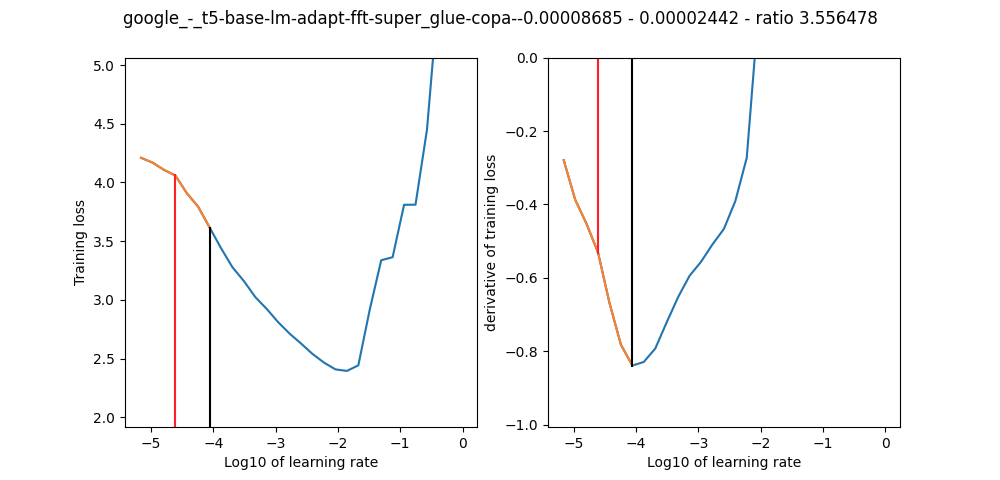
\includegraphics[width=0.4\textwidth]{example_optimization.png}
\caption{Optimization learning rate extraction for a FullFineTune model. Left: Loss versus learning rate. Right: Derivative of loss versus learning rate. Vertical black line is the optimal learning rate for training and the red line is the learning rate used for fine tuning.}
\label{example_optimization}
\end{figure}

\section{Results}
\begin{table*}[!htbp]
    \centering 
    \begin{tabular}{c c c c c c} 
        \\[-1.8ex]\hline \hline \\
        Benchmark & Task & FullFineTune & PromptTuning & SPoT Oracle & LibraryPrompt \\ 
        \hline \\[-1.8ex]
        GLUE & - & 71 & 69 & - & - \\ 
        SuperGLUE & - & 69 & 55 & 66 & 65 \\ 
        \hline \\[-1.8ex]
        GLUE & Cola & 55 & 51 & - & - \\ 
        GLUE & MNLI & 59 & 39 & - & - \\
        GLUE & MRPC & 87 & 87 & - & - \\
        GLUE & QNLI & 85 & 86 & - & - \\
        GLUE & QQP & 69 & 73 & - & - \\
        GLUE & RTE & 71 & 61 & - & - \\
        GLUE & SST2 & 91 & 92 & - & - \\
        GLUE & WNLI & 48 & 66 & - & - \\
        SuperGLUE & BoolQ & 79 & 63 & 67 & 74 \\
        SuperGLUE & CB & 93 & 72 & 77 & 84 \\
        SuperGLUE & Copa & 47 & 45 & 52 & 45 \\
        SuperGLUE & MultiRC & 63 & 52 & 54 & 61 \\
        SuperGLUE & WIC & 72 & 51 & 68 & 68 \\
        SuperGLUE & WSC Fixed & 60 & 48 & 79 & 60 \\
    \hline 
    \hline \\[-1.8ex] 
    \end{tabular}
    \caption{Comparison of algorithm performance.}
    \label{final_results} 
\end{table*} 
The comparison of the different models is shown in Table \ref{final_results}. The baseline SuperGLUE benchmark with full fine tuning (FullFineTune)  is about 5\% lower than what was shown by \cite{lester_2021}. There could be a few reasons for this. We are not using all the tasks in the benchmark and have only shown results on a subset. We train all models for 30K steps as compared to 260K by \cite{lester_2021}. The implementation of the SuperGLUE WSC dataset was different from the implementation by \cite{raffel_2022}.  Comparing the performance of vanilla soft prompt tuning (PromptTuning) and fully fine tuned (FullFineTune) models on GLUE tasks, the performance is similar. On the other hand, there is a significant difference in performance between FullFineTune and PromptTuning on the SuperGLUE tasks.  Soft prompt transfer (SPoT Oracle) performs ten points better than PromptTuning on the SuperGLUE tasks but does not match the performance of the FullyFineTune model. Unlike \cite{lester_2021} we only use 8 total prompts as compared to the 16 source tasks that were used by their study. This is one potential source of the difference. The generalized soft prompt method (LibraryPrompt) has a similar performance to Soft prompt transfer (SPoT Oracle) for overall performance to the SuperGLUE tasks. Looking closer at the individual model performance, LibraryPrompt performs better or equivalent in most tasks except for Copa and WSC. The test dataset for Copa is small and the difference could simply be probabilistic.


\begin{figure*}[t]
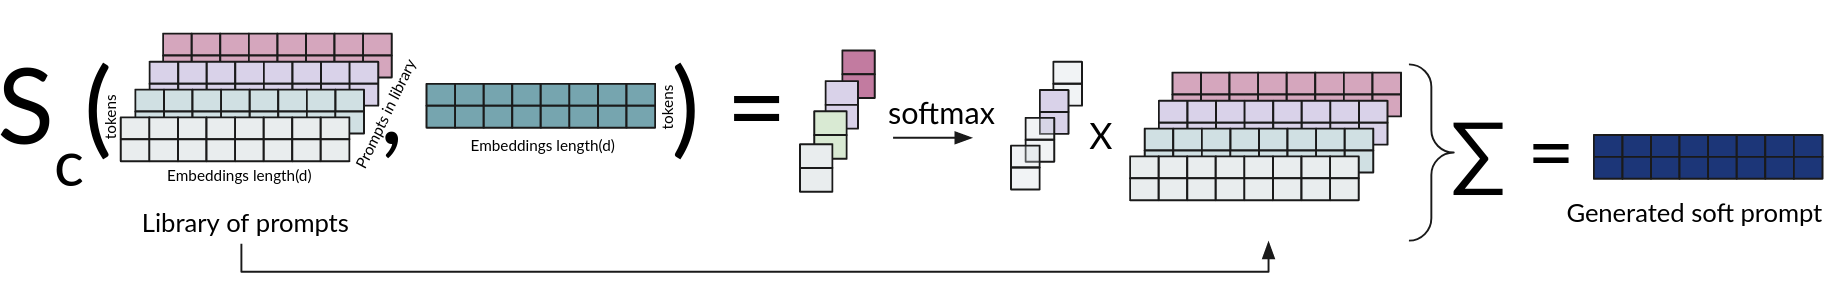
\includegraphics[width=\textwidth]{softmax.png}
\caption{Alternative library prompt using a token level softmax on the cosine similarity of a trained prompt with the library prompts.}
\label{softmax}
\centering
\end{figure*}

\section{Analysis}
Consider the LibraryPrompt architecture shown in Figure \ref{library_prompts_cross_weights}. The minimal set of weights required for a retrieval of a task is to provide each prompt an independent weight value and freeze the library. With this setup we make the tuning task as one of the tasks already in the library. Specifically, we pick the GLUE MRPC task. If the retrieval system works as expected, we would expect the weight associated with the MRPC prompt in the library to be dominant. The weights were initialized to 0.125, i.e. $\frac{1}{\text{Number of Prompts}}$ to ensure no bias was introduced at the start of training.

Figure \ref{prompt_weight_vs_iterations} demonstrates that the MRPC library weights quickly dominate and then settle down to a lower value. The initial overshoot of MRPC is likely because the MRPC tokens must overcome the weights of the other tokens and hence need to be that many times bigger than the rest. As the other token weights move towards 0, the MRPC weight also reduces proportionally. Note that in this implementation the generated token embeddings can only be a linear combination of the library tokens. This is a restrictive setup and does not extend well when training to new tasks but is shown as a step towards the final architecture shown in Figure \ref{library_prompts_cross_weights}.

\begin{figure}
\centering
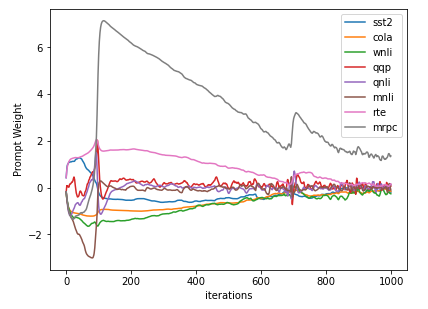
\includegraphics[width=0.4\textwidth]{prompt_weight_vs_iterations.png}
\caption{For a GLUE MRPC training task, the weight assiciated with the MRPC task in the prompt library quickly starts to dominate.}
\label{prompt_weight_vs_iterations}
\end{figure}

\section{Other Architectures}
We evaluated two architectures, one of the architectures was described earlier in Figure \ref{library_prompts_cross_weights} and the alternative is shown in Figure \ref{softmax}. This more complex architecture was our starting point as it is conceptually closer to the cosine similarity method used by \cite{vu_2022}. In this architecture, a set of weights (similarity weights) in the same shape as a prompt (number of tokens $\times$ embedding length) are trained. The generated prompt tokens use the following method. A cosine similarity is determined between each token of the library prompt and the similarity weights. A softmax of the library prompt is then performed in the axis of the tokens. This produces a matrix of probabilities (of size number of prompts $\times$ the number of tokens) where the sum across the tokens would add up to 1 due to the softmax operation. This probability matrix is multiplied with the library of prompt and summed across the token axis to produce the generated tokens.

The performance of the two architectures is shown in Table \ref{wa_vs_softmax}. Overall the weighted average architecture shown in Figure \ref{library_prompts_cross_weights} performs better than this softmax architecture.

\begin{table}[!htbp]
    \centering 
    \begin{tabular}{c c c} 
        \\[-1.8ex]\hline 
        \hline \\
        Task & LibraryPrompt(WA) & LibraryPrompt(SM) \\ 
        \hline \\[-1.8ex] 
    Average & 67 & 61.5 \\
    BoolQ & 73 & 60 \\
    CB & 83 & 68 \\
    Copa & 45 & 57 \\
    WIC & 67 & 61 \\  
    \hline 
    \hline \\[-1.8ex] 
    \end{tabular}
    \caption{Performance comparison of the softmax architecture in Figure \ref{softmax} with the weighted average architecture in Figure \ref{library_prompts_cross_weights}.}
    \label{wa_vs_softmax} 
\end{table} 


\section{Conclusion and Future Work}
We found that on average LibraryPrompt performed as well as SPoT on the chosen SuperGLUE tasks, which shows that there is a lot of potential for a generalized strategy for soft prompt tuning. Due to time constraints we were only able to experiment with two architectures (Weighted average and Softmax), but given the potential found here, it’s possible that other architectures could perform even better.
Having said that, even though the results from LibraryPrompt are promising, the performance of the fully fine tuned model and the Soft Prompt Transfer was not matched with previously published work. Several factors could have contributed to this, which have been previously listed. We would like to repeat this work with conditions that match previous work much more closely and hence can reproduce those results more faithfully. We would then like to compare the performance of LibraryPrompt with that baseline.

\appendix
\bibliographystyle{elsarticle-harv} 
\bibliography{example}

\newpage
\onecolumn
\section*{Appendix}

\textbf{Full Fine Tuning Data Preparation } \\

\begin{table}[!htbp]
    \centering
    \begin{tabularx}{\textwidth}{l l X l} 
        \\[-1.8ex]\hline 
        \hline \\
        Benchmark & Task & Processed Input & Process Output \\ 
        \hline \\[-1.8ex]
        SuperGLUE & CB & cb hypothesis: the language was peeled down. premise: It was a complex language. Not written down but handed down. One might say it was peeled down. & entailment \\
        SuperGLUE & MultiRC & multirc question: What did the high-level effort to persuade Pakistan include?. paragraph: While this process moved along, diplomacy continued its rounds. Direct pressure on the Taliban had proved unsuccessful. As one NSC staff note put it, "Under the Taliban, Afghanistan is not so much a state sponsor of terrorism as it is a state sponsored by terrorists." In early 2000, the United States began a high-level effort to persuade Pakistan to use its influence over the Taliban. In January 2000, Assistant Secretary of State Karl Inderfurth and the State Department\'s counterterrorism coordinator, Michael Sheehan, met with General Musharraf in Islamabad, dangling before him the possibility of a presidential visit in March as a reward for Pakistani cooperation. Such a visit was coveted by Musharraf, partly as a sign of his government\'s legitimacy. He told the two envoys that he would meet with Mullah Omar and press him on  Bin Laden. They left, however, reporting to Washington that Pakistan was unlikely in fact to do anything," given what it sees as the benefits of Taliban control of Afghanistan." President Clinton was scheduled to travel to India. The State Department felt that he should not visit India without also visiting Pakistan. The Secret Service and the CIA, however, warned in the strongest terms that visiting Pakistan would risk the President\'s life. Counterterrorism officials also argued that Pakistan had not done enough to merit a presidential visit. But President Clinton insisted on including Pakistan in the itinerary for his trip to South Asia. His one-day stopover on March 25, 2000, was the first time a U.S. president had been there since 1969. At his meeting with Musharraf and others, President Clinton concentrated on tensions between Pakistan and India and the dangers of nuclear proliferation, but also discussed  Bin Laden. President Clinton told us that when he pulled Musharraf aside for a brief, one-on-one meeting, he pleaded with the general for help regarding  Bin Laden." I offered him the moon when I went to see him, in terms of better relations with the United States, if he\'d help us get  Bin Laden and deal with another issue or two." The U.S. effort continued.' & False \\
    \hline 
    \hline \\[-1.8ex] 
    \end{tabularx}
    \label{data_prep} 
\end{table}


\begin{table}[!htbp]
    \centering
    \begin{tabularx}{\textwidth}{l l X l} 
        \\[-1.8ex]\hline 
        \hline \\
        Benchmark & Task & Processed Input & Process Output \\ 
        \hline \\[-1.8ex]
        SuperGLUE & BoolQ & boolq  passage: Persian language -- Persian (/ˈpɜːrʒən, -ʃən/), also known by its endonym Farsi (فارسی fārsi (fɒːɾˈsiː) ( listen)), is one of the Western Iranian languages within the Indo-Iranian branch of the Indo-European language family. It is primarily spoken in Iran, Afghanistan (officially known as Dari since 1958), and Tajikistan (officially known as Tajiki since the Soviet era), and some other regions which historically were Persianate societies and considered part of Greater Iran. It is written in the Persian alphabet, a modified variant of the Arabic script, which itself evolved from the Aramaic alphabet. question: do iran and afghanistan speak the same language. & True \\
        SuperGLUE & WIC & wic sentence1: Do you want to come over to my place later?. sentence2: A political system with no place for the less prominent groups. word: place & False \\
        SuperGLUE & Copa & copa choice1: The sun was rising. choice2: The grass was cut. premise: My body cast a shadow over the grass. question: cause. & choice1 \\
        SuperGLUE & WSC & wsc.fixed paragraph: *Mark* told Pete many lies about himself, which Pete included in his book. *He* should have been more skeptical. & false \\
        GLUE & RTE & rte hypothesis: Christopher Reeve had an accident. premise: Dana Reeve, the widow of the actor Christopher Reeve, has died of lung cancer at age 44, according to the Christopher Reeve Foundation. & not\_entailment \\
        GLUE & MNLI & mnli hypothesis: Product and geography are what make cream skimming work. premise: Conceptually cream skimming has two basic dimensions - product and geography. & neutral \\
        GLUE & Cola & cola sentence: Our friends won't buy this analysis, let alone the next one we propose. & acceptable \\
        GLUE & MRPC & mrpc sentence1: Amrozi accused his brother , whom he called " the witness " , of deliberately distorting his evidence . sentence2: Referring to him as only " the witness " , Amrozi accused his brother of deliberately distorting his evidence . & not\_equivalent \\
        GLUE & QNLI & qnli sentence: Unlike the two seasons before it and most of the seasons that followed, Digimon Tamers takes a darker and more realistic approach to its story featuring Digimon who do not reincarnate after their deaths and more complex character development in the original Japanese. question: When did the third Digimon series begin? & not\_entailment \\
        GLUE & QQP & qqp question1: How is the life of a math student? Could you describe your own experiences? question2: Which level of prepration is enough for the exam jlpt5? & not\_duplicate \\
        GLUE & SST2 & qqp question1: sst2 sentence: hide new secretions from the parental units. & negative \\
        GLUE & WNLI & wnli sentence1: The drain is clogged with hair. It has to be cleaned. sentence2: The hair has to be cleaned. & not\_entailment \\
    \hline 
    \hline \\[-1.8ex] 
    \end{tabularx}
    \label{data_prep} 
\end{table} 

\newpage

\textbf{Prompt Methods Data Preparation} \\
The prompt method data preparation matches the previous section except that all inputs are appended with the word absence repeated 20 times and the task name is not appended to the task. Here is an example for WNLI:

\begin{table}[!htbp]
    \centering
    \begin{tabularx}{\textwidth}{l l X l} 
        \\[-1.8ex]\hline 
        \hline \\
        Benchmark & Task & Processed Input & Process Output \\ 
        \hline \\[-1.8ex]
        GLUE & WNLI & absence  absence  absence  absence  absence  absence  absence  absence  absence  absence  absence  absence  absence  absence  absence  absence  absence  absence  absence  absence  sentence1: The drain is clogged with hair. It has to be cleaned. sentence2: The hair has to be cleaned. & not\_entailment \\
    \hline 
    \hline \\[-1.8ex] 
    \end{tabularx}
    \label{data_prep} 
\end{table}


%% If you have bibdatabase file and want bibtex to generate the
%% bibitems, please use
%%


%% else use the following coding to input the bibitems directly in the
%% TeX file.

%%\begin{thebibliography}{00}

%% \bibitem[Author(year)]{label}
%% Text of bibliographic item

%%\bibitem[ ()]{}

%%\end{thebibliography}
\end{document}

\endinput
%%
%% End of file `elsarticle-template-harv.tex'.
